% CAPÍTULO 5: METODOLOGÍA DE DESARROLLO

\chapter{Metodología de desarrollo}
\label{cap:metodologia}

En este capítulo se detalla el marco metodológico utilizado para el desarrollo y
despliegue del Sistema Inteligente para la Identificación y Seguimiento
de NNAs por feminicidios. Debido a la alta complejidad algorítmica asi como la alta
incertidumbre tecnológica del proyecto (particularmente en las fases de validación
de modelos de lenguaje) se adoptó un enfoque \textbf{evolutivo} que garantizaba
la dirección hacia una solución correcta y de calidad de producción mediante
retroalimentación empírica continua.

\section{Metodología de desarrollo evolutivo}
\label{sec:met_evolutivo}

Se seleccionó el modelo de desarrollo evolutivo basado en prototipos como base del proceso
fundamental para guiar el ciclo de vida del software. Esta decisión responde a dos razones
técnicas no negociables que son asociadas a la alta incertidumbre en las fronteras de la
ingesta de datos y el aprendizaje del lenguaje natural.

\begin{enumerate}
    \item \textbf{Incertidumbre en la ingesta de datos.} El ecosistema web contemporáneo
    emplea infraestructuras dinámicas de seguridad y mitigación de amenazas (WAF, \textit{bot detection} avanzado
    y \textit{JA3/TLS fingerprinting}) que alteran sus políticas y firmas de forma impredecible. Ante la inexistencia
    de APIs públicas centralizadas para la nota roja local, era imposible determinar qué mecanismos de recolección
    sintáctica tendrían éxito sin iterar y ajustar el código para mejorar el ratio de éxito.
    \item \textbf{Incertidumbre algorítmica en el Procesamiento de Lenguaje Natural (\textit{NLP}).} El salto desde la rigidez
    determinista de los enfoques léxicos (expresiones regulares) hacia la flexibilidad semántica abstracta del aprendizaje profundo
    introdujo variables de estocasticidad que impactan directamente la precisión. La instrumentación de modelos fundacionales
    basados en atención (\textit{Transformers}) demandó un ciclo de vida donde cada iteración fungia como un entorno de diagnóstico.
    Mitigar el ruido temático y fenómenos complejos como el \textit{"efecto péndulo"} requeria aislar las colisiones semánticas
    calibrando parámetros mediante estrategias de ajuste fino (\textit{Fine-tuning}).
\end{enumerate}

\subsection{Cronograma general de evolución del proyecto}
\label{subsec:met_cronograma}

El ciclo de vida abarcó dos semestres académicos estructurados de forma secuencial:

\begin{description}
    \item[\textbf{Fase Trabajo Terminal I (Sep-Dic 2025)}] Validación de viabilidad técnica y establecimiento de la línea base mediante que explorana la ingesta sintáctica (\texttt{P0} a \texttt{P2}).
    El énfasis metodológico consistió en demostrar la capacidad de extracción de información  web de forma automatizada a escala sobre medios digitales locales y poder confirmar que las aproximaciones
    heurísticas resultaban insuficientes ante el lenguaje periodístico policial mexicano.
    \item[\textbf{Fase Trabajo Terminal II (Feb-Jun 2026)}] Optimización de Machine Learning, consolidación de la arquitectura híbrida y despliegue de grado producción (\texttt{P3} y \texttt{P4}).
    El esfuerzo se concentró en resolver el ruido semántico de la fase previa mediante el ajuste local del modelo Transformer \textbf{BETO}enriquecido
    con tecnicas de disminución de ruido semántico lo que estabilizaba el sistema mediante un algoritmo de clasificación escalonada y una arquitectura de software escalable
    mediante contenedores Docker.
    \end{description}

\begin{figure}[H]
    \centering
    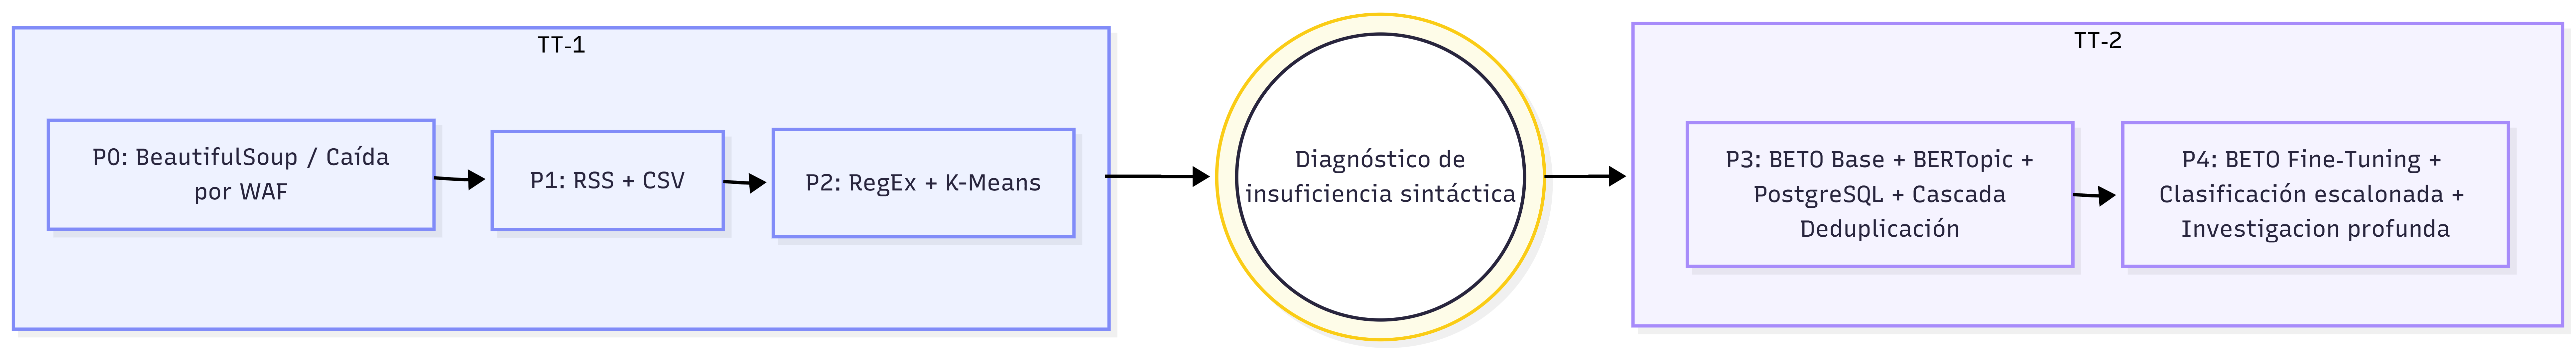
\includegraphics[width=\textwidth]{images/cronograma.png}
    \caption{Cronograma metodológico de evolución y transición de los prototipos del sistema.}
    \label{fig:cronograma_evolucion}
\end{figure}

\section{Evolución metodológica de los prototipos} 
\label{sec:met_evolucion_prototipos}

El ciclo de vida del sistema se rigió mediante un enfoque incremental donde cada prototipo actuó como un entorno de diagnóstico. Las limitaciones, los desbordamientos de memoria y las colisiones
semánticas medidas en las fases tempranas impulsaron directamente el diseño y la reconfiguración para las soluciones avanzadas de la fase final.

\subsection{Fase TT-1 Prototipos exploratorios e ingesta sintáctica (P0-P2)}
\label{subsec:met_tt1_prototipos}

\begin{description}
    \item[\textbf{Prototipo 0 (P0) Ingesta directa y fracaso rápido} \textit{(Sep 2025)}.] 
          Implementación inicial de extracción de noticias empleando \texttt{BeautifulSoup} sobre peticiones HTTP directas. 
          \textit{Resultado:} Bloqueos perimetrales sistemáticos por parte de firewalls de aplicación web (WAF como Cloudflare) con códigos de estado HTTP 403 en el 80\% de las fuentes objetivo. 
          \textit{Conclusión:} El \textit{fingerprinting TLS} nativo de la biblioteca \texttt{requests} resulta fácilmente identificable por sistemas antibot modernos. 
          \textit{Decisión:} Abandonar el raspado HTML directo no autenticado como estrategia de ingesta primaria.

    \item[\textbf{Prototipo 1 (P1): Ingesta mediante feeds RSS} \textit{(Oct 2025)}.]  
          Cambio de estrategia hacia canales de distribución de noticias por medio de RSS de 10 medios de comunicación de cobertura nacional implementado con persistencia estructurada en archivos
          planos CSV mediante \texttt{Pandas}. 
          \textit{Resultado:} Recolección exitosa de 200 registros de texto en el primer ciclo mensual con una tasa de bloqueo del 0\%. 
          \textit{Limitación:} Sesgo de cobertura mediática (exclusión de portales locales sin RSS público) y carencia absoluta de mecanismos de extracción semántica o discriminación temática.

    \item[\textbf{Prototipo 2 (P2): Clasificación heurística y clustering estadístico} \textit{(Nov-Dic 2025)}.] 
          Diseño de un clasificador basado en expresiones regulares (RegEx con 47 patrones sintácticos) para identificación de entidades, acoplado a un clasificador
          estadístico disperso mediante vectorización TF-IDF y agrupamiento K-Means ($k=8$ estático). 
          \textit{Resultado:} Margen de error superior al 60\% en la detección de casos relevantes, principalmente tres escenarios críticos de colisión como notas legislativas o estadísticas
          de violencia de género sin casos objetivos de violencia.
          \textit{Diagnóstico:} El enfoque sintáctico era incapaz de identificar la relación conceptual entre términos o resolver dependencias de largo alcance en textos no estructurados.
\end{description}

\subsection{Fase TT-2 Arquitectura de aprendizaje profundo y clasificador escalonado (P3-P4)}
\label{subsec:met_tt2_prototipos}

\begin{description}
    \item[\textbf{Prototipo 3 (P3) Inferencia semántica base y migración relacional} \textit{(Feb-Mar 2026)}.] 
          Sustitución de las heurísticas rígidas por un clasificador Transformer discriminativo basado en el modelo de lenguaje \textbf{BETO} base que operaba inicialmente
          bajo una estrategia de proximidad semántica por similitud coseno y la migración de la capa de almacenamiento hacia un motor relacional en PostgreSQL. Implementación
          del flujo de de-duplicación en cascada de 4 capas (MD5 $\rightarrow$ SimHash $\rightarrow$ Jaccard $\rightarrow$ coseno TF-IDF) e integración de la biblioteca
          \texttt{StealthSession} con emulación de JA3 fingerprinting. 
          \textit{Resultado:} Reducción del ruido léxico al 20\% y expansión del catálogo de monitoreo a 45 fuentes web correlativas.  
          \textit{Limitación:} Aparición del \textit{"efecto péndulo"} donde el clasificador Transformer exhibía una alta afinidad semántica
          por cercanía léxica lo que hacía que clasificara erróneamente discursos normativos (como iniciativas de la Ley Monzón) o reportes
          institucionales (como cifras de REDIM) como eventos delictivos reales debido a la coincidencia masiva de tokens comunes.

    \item[\textbf{Prototipo 4 (P4) Fine-tuning optimizado, clasificador escalonado y dashboard} \textit{(Abr-Jun 2026)}.] 
          Evolución hacia el estado actual de producción del sistema mediante tres aspectos fundamentales de ingeniería de software y machine learning.
          \begin{enumerate}
              \item \textbf{Fine-tuning local:} Entrenamiento de las capas de clasificación de BETO utilizando un dataset etiquetado manualmente con los casos positivos reales clasificados en el Prototipo 3.
              El proceso incorporó técnicas de optimización para mitigar las restricciones de cómputo (8 GB de RAM).
              \item \textbf{Sistema de clasificación escalonado:} Estabilización del clasificador mediante una arquitectura de decisión híbrida en 3 capas que fue el escudo léxico duro,
              el filtro temático (aplicación de penalizaciones suaves de $-0.35$ para neutralizar el efecto péndulo), inferencia fina del Transformer ajustado y bonificaciones heurísticas
              sintácticas para la detección de parentescos ($+0.10$ a $+0.25$).
          \end{enumerate}
          \textit{Resultado:} Plataforma robusta con una precisión alta en la identificación de casos relevantes y lista para su adopción operativa por colectivos de búsqueda y organizaciones de derechos humanos.
\end{description}


\section{Evolución del Stack Tecnológico (TT-1 \texorpdfstring{$\rightarrow$}{->} TT-2)} 
\label{sec:met_stack}

La maduración iterativa del sistema forzó una refactorización integral de las dependencias de software y los paradigmas algorítmicos: cada limitación de exactitud o desbordamiento de memoria medido en TT-1 motivó directamente una decisión arquitectónica en TT-2. La Tabla~\ref{tab:stack_evolucion} sistematiza esta evolución por capa arquitectónica, documentando formalmente el cuello de botella superado y la transición hacia un pipeline de grado producción con aprendizaje profundo optimizado.

\begin{table}[H]
\centering
\caption{Evolución del Stack Tecnológico e Ingeniería de Optimización (TT-1 vs TT-2)}
\label{tab:stack_evolucion}
\begin{tabular}{|p{2.8cm}|p{5.0cm}|p{5.2cm}|}
\hline
\textbf{Capa} &
\textbf{TT-1 (Prototipo 2)} &
\textbf{TT-2 (Prototipo 4 Consolidado)} \\
\hline
\textbf{Lenguaje base} &
Python 3.10, scripts secuenciales en CLI sin abstracción de datos. &
Python 3.11, pipeline asíncrono y modular estructurado bajo el patrón de diseño \textit{Repository Pattern}. \\
\hline
\textbf{Recolección} &
10 fuentes RSS mediante la biblioteca \texttt{requests} (vulnerable a bloqueos por estructura HTML). &
45 fuentes RSS automatizadas + Google News API + \texttt{StealthSession} v7.0 con emulación de \textit{JA3 fingerprinting} y evasión perimetral. \\
\hline
\textbf{Persistencia} &
Archivos planos CSV manejados con Pandas; carencia de acceso concurrente e integridad referencial. &
PostgreSQL 16 + SQLAlchemy ORM; soporte ACID/MVCC e indexación GIN especializada para Búsqueda de Texto Completo (\textit{FTS}) en español. \\
\hline
\textbf{Clasificación NLP y Machine Learning} &
RegEx rígido (47 patrones sintácticos) y similitud estadística TF-IDF; alta tasa de falsos positivos ($>18.6\%$). &
\textbf{BETO Fine-tuned} mediante \textit{Active Learning} con inyección de \textit{Hard Negatives}. Arquitectura Transformer discriminativa para sintaxis relacional profunda. \\
\hline
\textbf{Optimización de Cómputo (Hardware)} &
No requerida; los scripts heurísticos operaban con bajo consumo de memoria volátil. &
\textbf{Linear Probing} estricto (congelamiento de las capas 0-11 del encoder de BETO, $\text{parámetros entrenables} = 0.2\%$) y \textbf{Acumulación de Gradientes} (\texttt{accum=8}, \texttt{batch=4}) para entrenamiento local en 8 GB de RAM sin fallos \textit{OOM}. \\
\hline
\textbf{Agrupamiento (Clustering)} &
Algoritmo K-Means ($k$ estático) sobre vectores dispersos TF-IDF; clústeres semánticamente incoherentes. &
BERTopic con \textbf{resiliencia matemática defensiva}: ajuste dinámico de \texttt{CountVectorizer(min\_df=1)} ante corpus reducidos para neutralizar colapsos por \textit{ValueError}. \\
\hline
\textbf{Deduplicación} &
Validación binaria simple mediante comparación de URLs exactas. &
Cascada estocástica de 4 fases correlativas: hashing MD5 $\rightarrow$ SimHash de contenido $\rightarrow$ distancia Jaccard $\rightarrow$ coseno TF-IDF. \\
\hline
\textbf{Lógica de Decisión (Inference)} &
Lógica binaria determinista basada puramente en coincidencias de expresiones regulares. &
\textbf{Sistema de Scoring Escalonado (Tiered Scoring v7.1)} en 4 capas concurrentes: Escudo Léxico, Filtro Temático No-Fáctico (penalización suave de $-0.35$), Inferencia BETO y Bonificaciones Heurísticas Sintácticas ($+0.10$ a $+0.25$). \\
\hline
\textbf{Despliegue} &
Scripts CLI locales; dependencia absoluta de las variables del entorno del desarrollador. &
Orquestación multifase mediante Docker Compose (3 contenedores independientes); servidor WSGI Gunicorn; red aislada tipo \textit{bridge}. \\
\hline
\textbf{Interfaz y Consumo} &
Inexistente; persistencia y depuración directa sobre la consola estándar y archivos intermedios. &
Dashboard web interactivo en Flask + API REST integrada; visualización analítica de fichas de caso extraídas y gestión CRUD de fuentes de información. \\
\hline
\end{tabular}
\end{table}

%----------------------------------------------------------------------------------------
\section{Arquitectura de Microservicios, Contenerización y Gestión de Recursos}
\label{sec:met_arquitectura_docker}
%----------------------------------------------------------------------------------------

La culminación del Prototipo 4 consolidó un ecosistema distribuido definido mediante una orquestación en \texttt{docker-compose.yml} y regido por el principio de aislamiento arquitectónico y separación de responsabilidades (\textit{Separation of Concerns}). Debido a la severa restricción de hardware local del entorno de operación (límite estricto de 8 GB de RAM), la arquitectura se diseñó no solo para asegurar el aislamiento de fallos, sino para actuar como un regulador estricto del consumo de memoria volátil. El sistema se organiza en tres contenedores independientes que se comunican de forma exclusiva sobre una red virtual \textit{bridge} privada (\texttt{nna-network}), garantizando que los picos de cómputo durante la inferencia y el minado de datos no desestabilicen el sistema operativo anfitrión.

\subsection{Contenedor de Base de Datos y Persistencia Relacional: \texttt{nna-postgres}}
\label{subsec:met_contenedor_postgres}

El contenedor \texttt{nna-postgres} ejecuta el motor relacional \textbf{PostgreSQL 16 Alpine} (\texttt{postgres:16-alpine}), seleccionando una imagen minimizada de 78~MB para maximizar la disponibilidad de RAM para las capas de Aprendizaje Profundo. Su configuración y políticas de persistencia incluyen:

\begin{itemize}
    \item \textbf{Volumen persistente de grado producción:} El volumen lógico \texttt{pgdata} se monta directamente en la ruta nativa \texttt{/var/lib/postgresql/data}, garantizando la persistencia, atomicidad y supervivencia de los registros estructurados de las víctimas y las tablas analíticas ante reinicios o reconstrucciones del contenedor.
    \item \textbf{Sincronización jerárquica de servicios (Healthcheck):} Implementa una directiva de verificación de estado mediante el comando \texttt{pg\_isready -U postgres}. Los contenedores dependientes de la lógica de negocio (\texttt{nna-analyzer} y \texttt{nna-webapp}) tienen bloqueado su despliegue hasta que este sub-sistema declare un estado saludable, erradicando por completo las condiciones de carrera (\textit{race conditions}) en la inicialización de sockets de red.
    \item \textbf{Seguridad perimetral interna:} El puerto nativo 5432 se expone de manera exclusiva hacia la red interna aislada \texttt{nna-network}. Al no mapear este puerto hacia la interfaz pública del host de producción, se reduce a cero la superficie de ataque por inyección o escaneo de puertos externo.
\end{itemize}

\subsection{Contenedor del Motor de Ingesta e Inferencia Machine Learning: \texttt{nna-analyzer}}
\label{subsec:met_contenedor_analyzer}

El contenedor \texttt{nna-analyzer} encapsula la inteligencia del backend, ejecutando el pipeline periódico estructurado mediante un planificador modular. Este módulo gestiona de forma nativa los procesos críticos del ciclo de vida del dato: recolección (Web Scraping masivo), preprocesamiento, deduplicación multidimensional e inferencia Transformer. Sus características de diseño metodológico son:

\begin{itemize}
    \item \textbf{Persistencia y persistencia de pesos (Caché de Modelos):} Incorpora un volumen compartido denominado \texttt{models\_cache} montado en \texttt{/app/models/cache}. Los pesos del modelo encoder \textbf{BETO Fine-tuned} ($\approx$440~MB) se almacenan de manera local y determinista. Las variables de entorno de la biblioteca Hugging Face (\texttt{TRANSFORMERS\_CACHE} y \texttt{HF\_HOME}) se redirigen hacia este volumen, neutralizando la latencia de red y evitando descargas redundantes en cada ciclo de vida del contenedor.
    \item \textbf{Acoplamiento y mitigación de fallos de red:} Posee una dependencia condicional estricta configurada mediante \texttt{depends\_on} asociada al estado \texttt{service\_healthy} de \texttt{nna-postgres}. Esto garantiza la resiliencia del pipeline de datos, impidiendo que los hilos de raspado web inicien si el pool de conexiones de la base de datos no está disponible para la persistencia inmediata.
    \item \textbf{Programación Defensiva y Ajuste Dinámico:} Aloja las configuraciones del pipeline híbrido, incluyendo los parámetros de resiliencia del módulo de clustering \texttt{BERTopic}. Al parametrizar de forma dinámica el tokenizador del sub-modelo de representación léxica (\texttt{CountVectorizer(min\_df=1)}), el contenedor previene de manera proactiva colapsos de ejecución (\textit{ValueError}) cuando los lotes periódicos de noticias recolectadas sufren una contracción crítica de volumen.
\end{itemize}

\subsection{Contenedor de Interfaz Analítica y Dashboard Web: \texttt{nna-webapp}}
\label{subsec:met_contenedor_webapp}

El contenedor \texttt{nna-webapp} sirve el Dashboard interactivo y la interfaz de control mediante el micro-framework Flask, orquestado bajo el servidor de aplicaciones WSGI de grado producción \textbf{Gunicorn}. Debido a las restricciones físicas de memoria (8 GB de RAM del equipo anfitrión), la parametrización de este contenedor se calibró minuciosamente para evitar colisiones con las fases de entrenamiento local:

\begin{itemize}
    \item \textbf{Modelado de Concurrencia Restringido:} Se configuró la ejecución estricta de \textbf{2 workers} Gunicorn basados en un modelo de subprocesos \textit{pre-forked} (\texttt{--workers 2}). Esta decisión arquitectónica limita deliberadamente la concurrencia a un máximo de dos solicitudes HTTP pesadas simultáneas. Aunque esto limita el rendimiento de red a gran escala, garantiza que el consumo base de RAM del contenedor se estabilice en un umbral mínimo, reservando el espacio libre de la memoria para que el script de re-entrenamiento local (\textit{Active Learning}) basado en \textit{Linear Probing} y acumulación de gradientes se ejecute en el host de forma segura y sin desbordamientos de memoria (\textit{Out Of Memory}).
    \item \textbf{Calibración de Timeouts para Inferencia en CPU:} Se determinó un límite de tiempo de respuesta extendido de 300 segundos (\texttt{--timeout 300}). Esta holgura está metodológicamente justificada debido a que la evaluación semántica y las consultas de investigación profunda \textit{on-demand} (\texttt{DeepInvestigator}) se procesan exclusivamente utilizando la CPU del host, lo que puede elevar los tiempos de cómputo en lotes densos; un timeout estándar (30 s) provocaría la terminación prematura y destructiva del hilo de análisis por parte de Gunicorn.
    \item \textbf{Consumo Descentralizado y API REST:} Expone de forma exclusiva el puerto 5000 hacia el host. Este diseño permite que la interfaz web y la API REST pública actúen como la capa de abstracción final, aislando al usuario investigador de la complejidad algorítmica del backend y asegurando un canal limpio para la auditoría de los datos estructurados.
\end{itemize}
%----------------------------------------------------------------------------------------
\section{Especificación de Requerimientos y Matriz de Trazabilidad Evolutiva}
\label{sec:met_trazabilidad_prototipos}
%----------------------------------------------------------------------------------------

La formalización y el diseño de la arquitectura distribuida fueron gobernados por un conjunto estricto de requerimientos funcionales (RF) y no funcionales (RNF), cuyos criterios de aceptación e hitos de ingeniería se validaron empíricamente bajo el paradigma de prototipado incremental. Con la finalidad de garantizar el rigor metodológico del proyecto, la Tabla~\ref{tab:trazabilidad_prototipos} sistematiza la matriz de trazabilidad general. Este instrumento documenta la cobertura incremental y la evolución de cada directiva de software a lo largo del ciclo de vida, demostrando analíticamente cómo el sistema convergió hacia una cobertura del 100\% en el Prototipo 4 consolidado.

\begin{table}[H]
\centering
\caption{Matriz de Trazabilidad General: Requerimientos de Software vs. Prototipos Evolutivos}
\label{tab:trazabilidad_prototipos}
\begin{tabular}{|p{1.4cm}|p{6.4cm}|c|c|c|c|c|}
\hline
\textbf{ID} &
\textbf{Especificación del Requerimiento} &
\textbf{P0} &
\textbf{P1} &
\textbf{P2} &
\textbf{P3} &
\textbf{P4} \\
\hline
\textbf{RF-01} &
Extracción multi-fuente enfocada mediante técnicas de \textit{web scraping} asíncrono con evasión perimetral anti-bot. &
$\sim$ & \checkmark & \checkmark & \checkmark & \checkmark \\
\hline
\textbf{RF-02} &
Deduplicación estocástica y lógica en cascada multidimensional (MD5 $\rightarrow$ SimHash $\rightarrow$ Jaccard $\rightarrow$ coseno TF-IDF). &
--- & --- & $\sim$ & \checkmark & \checkmark \\
\hline
\textbf{RF-03} &
Clasificación semántica binaria profunda mediante el modelo Transformer \textbf{BETO Fine-tuned} localmente a nivel de tokens relacionales. &
--- & --- & --- & $\sim$ & \checkmark \\
\hline
\textbf{RF-04} &
Mitigación de colisiones léxicas (\textit{Efecto Péndulo}) mediante un algoritmo híbrido de Puntuación Escalonada (\textit{Tiered Scoring v7.1}). &
--- & --- & --- & --- & \checkmark \\
\hline
\textbf{RF-05} &
Agrupamiento semántico latente y modelado automático de tópicos interactivos mediante la integración de \texttt{BERTopic}. &
--- & --- & --- & \checkmark & \checkmark \\
\hline
\textbf{RF-06} &
Persistencia híbrida distribuida (PostgreSQL relacional con indexación GIN + CSV intermedio) para auditoría e integridad referencial. &
--- & $\sim$ & $\sim$ & \checkmark & \checkmark \\
\hline
\textbf{RF-07} &
Dashboard administrativo web interactivo con el módulo \texttt{DeepInvestigator} para validación, exportación masiva y gestión CRUD de fuentes. &
--- & --- & --- & --- & \checkmark \\
\hline\hline
\textbf{RNF-01} &
\textbf{Eficiencia en Cómputo Local:} Ejecución del pipeline y re-entrenamiento mediante \textit{Linear Probing} y acumulación de gradientes en $\le$ 8 GB de RAM sin fallos \textit{OOM}. &
--- & --- & --- & --- & \checkmark \\
\hline
\textbf{RNF-02} &
\textbf{Resiliencia Matemática:} Tolerancia a fallos defensiva y parametrización dinámica en la capa de clustering ante contracciones críticas del corpus. &
--- & --- & --- & --- & \checkmark \\
\hline
\textbf{RNF-03} &
\textbf{Seguridad y Privacidad Ética:} Anonimización programática de infancias (cumplimiento LGDNNA) e integridad transaccional ACID de extremo a extremo. &
--- & --- & $\sim$ & \checkmark & \checkmark \\
\hline
\end{tabular}
\\
{\small \textit{Leyenda:} \checkmark = Requerimiento completamente satisfecho y validado; $\sim$ = Implementación parcial o en fase de pruebas unitarias; --- = No abordado / Fuera de la frontera de especificación de la fase.}
\end{table}

El análisis analítico de la matriz de trazabilidad evidencia la naturaleza evolutiva del proceso de desarrollo de software. Los prototipos iniciales (\texttt{P0} a \texttt{P2}) se concentraron exclusivamente en resolver la frontera de especificación sintáctica, garantizando la ingesta masiva de flujos web y la manipulación estructurada de datos planos. 

El salto cualitativo hacia el procesamiento profundo en el Prototipo 3 introdujo requerimientos semánticos de alta densidad neural, aislando las primeras colisiones lógicas provocadas por el solapamiento léxico de los discursos informativos. Finalmente, el Prototipo 4 resolvió categóricamente las exigencias más complejas de eficiencia computacional extrema en hardware restringido y resiliencia matemática algorítmica. Este hito cerró con éxito la cobertura total de la matriz, consolidando un ecosistema tecnológico maduro, auditable y robusto, listo para someterse a la validación científica y metodológica frente al sínodo académico.